\begin{figure}
    \centering
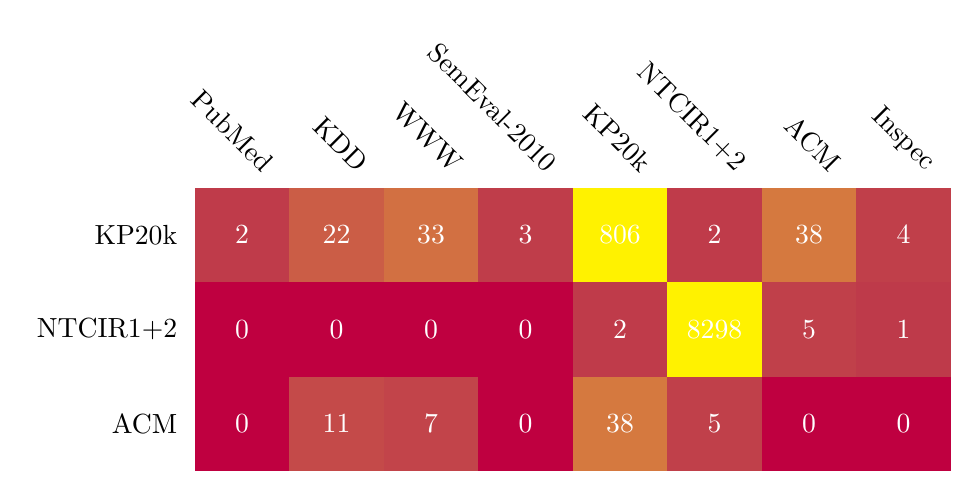
\begin{tikzpicture}[scale=1.2]
\foreach \x [count=\n] in {
        PubMed,KDD,WWW,SemEval-2010,KP20k,NTCIR1+2,ACM,Inspec
  } {
       \node[rotate=-45,xshift=0.6cm,anchor=east] at (\n,0) {\x};
  }
  \foreach \x [count=\n] in {
        KP20k,NTCIR1+2,ACM
  } {
       \node[xshift=0.5cm,anchor=east] at (0,-\n) {\x};
  }
  \foreach \y [count=\n] in {
        %{0,  0,   0, 0,  2,   0,  0,0},
        %{0,  0,   0, 0, 22,   0, 11,0},
        %{0,  0,   0, 0, 33,   0,  7,0},
        %{0,  0,   0, 0,  3,   0,  0,0},
        {2, 22,  33, 3,806,   2, 38,4},
        {0,  0,   0, 0,  2,8298,  5,1},
        {0, 11,   7, 0, 38,   5,  0,0},
        %{0,  0,   0, 0,  4,   1,  0,0},
    } {
      \foreach \x [count=\m] in \y {
        \node[fill=yellow!\x!purple, minimum size=12mm, text=white] at (\m,-\n) {\x};
      }
    }
\end{tikzpicture}
    \caption{Nombre de document commun entre les ensembles de test des jeux de données utilisés.}
    \label{fig:heatmap_test}
\end{figure}